\documentclass[tikz,border=6pt]{standalone}
\usepackage{amsmath,amssymb}
\usetikzlibrary{arrows.meta}
\begin{document}
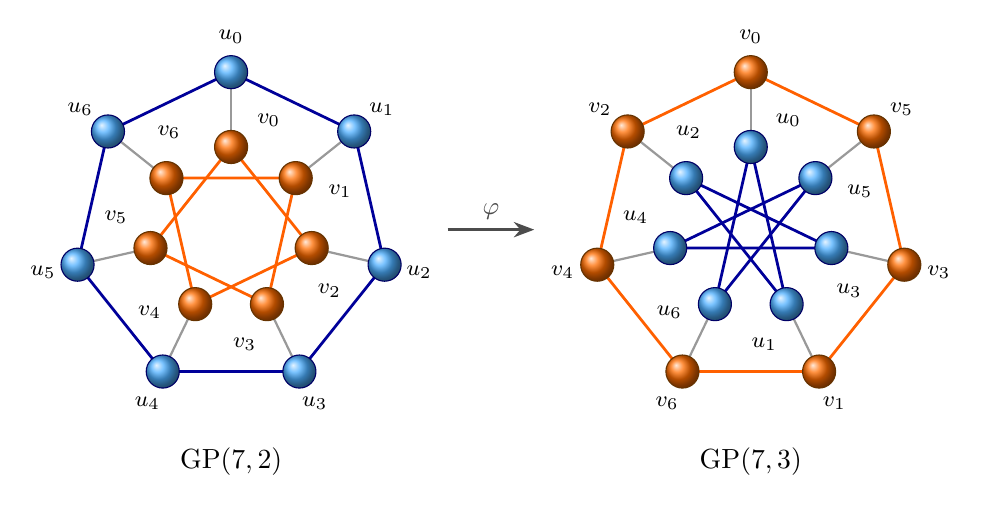
\begin{tikzpicture}[
  ub/.style={circle,shading=ball,ball color=blue!45!cyan!70,draw=blue!40!black,minimum size=4.2mm,inner sep=0pt},
  vo/.style={circle,shading=ball,ball color=orange!85!red,draw=orange!40!black,minimum size=4.2mm,inner sep=0pt},
  eb/.style={draw=blue!60!black,line width=1.0pt},
  eo/.style={draw=orange!75!red,line width=1.0pt},
  sp/.style={draw=black!40,line width=0.8pt},
  lab/.style={font=\footnotesize,inner sep=1pt}]
  \def\R{2.0}\def\r{1.05}
  % ---------- GP(7,2): u_i outside (blue), v_i inside (orange) ----------
  \begin{scope}
    \foreach \i in {0,...,6} {
      \coordinate (U\i) at ({90-360*\i/7}:\R);
      \coordinate (V\i) at ({90-360*\i/7}:\r);
    }
    \foreach \i [evaluate=\i as \j using {int(mod(\i+1,7))}, evaluate=\i as \k using {int(mod(\i+2,7))}] in {0,...,6} {
      \draw[sp] (U\i)--(V\i);
      \draw[eb] (U\i)--(U\j);
      \draw[eo] (V\i)--(V\k);
    }
    \foreach \i in {0,...,6} {
      \node[ub] at (U\i) {}; \node[vo] at (V\i) {};
      \node[lab] at ({90-360*\i/7}:{\R+0.45}) {$u_{\i}$};
      \node[lab] at ({90-360*\i/7-19}:1.47) {$v_{\i}$};
    }
    \node at (0,-2.95) {$\mathrm{GP}(7,2)$};
  \end{scope}
  % ---------- GP(7,3): vertex at outer position j is phi(v_{5j}), inner position j is phi(u_{5j}) ----------
  \begin{scope}[xshift=6.6cm]
    \foreach \i in {0,...,6} {
      \coordinate (A\i) at ({90-360*\i/7}:\R);
      \coordinate (B\i) at ({90-360*\i/7}:\r);
    }
    \foreach \i [evaluate=\i as \j using {int(mod(\i+1,7))}, evaluate=\i as \k using {int(mod(\i+3,7))}] in {0,...,6} {
      \draw[sp] (A\i)--(B\i);
      \draw[eo] (A\i)--(A\j);
      \draw[eb] (B\i)--(B\k);
    }
    \foreach \i [evaluate=\i as \m using {int(mod(5*\i,7))}] in {0,...,6} {
      \node[vo] at (A\i) {}; \node[ub] at (B\i) {};
      \node[lab] at ({90-360*\i/7}:{\R+0.45}) {$v_{\m}$};
      \node[lab] at ({90-360*\i/7-19}:1.47) {$u_{\m}$};
    }
    \node at (0,-2.95) {$\mathrm{GP}(7,3)$};
  \end{scope}
  \draw[-{Stealth[length=2.6mm]},line width=0.9pt,black!70] (2.75,0) -- node[above,font=\small] {$\varphi$} (3.85,0);
\end{tikzpicture}
\end{document}
